\chapter[Blur Resilient Fiducials]{A Motion Blur Resilient Fiducial For
Quadcopter Imaging}
\section{Introduction}

The recent availability of low-cost quadcopters has helped  fuel
significant efforts in research focused on unmanned aerial
vehicles. Navigation and planning
of these vehicles is typically~\cite{Davison:2007,Engel12,Engel13}
performed using onboard inertial sensors and/or vision based modules
that uses visual cues in the real world. However, to evaluate the
effectiveness of navigation methods, one or more fiducials are commonly
placed~\cite{Bosnak:2012,Lim09,Klopschitz:2007}
 in the environment to provide additional information that
serves for ground-truth positional measurements.

In order to be effective, fiducial markers (or simply, fiducials) need
to be easily detected in the scene. A variety of fiducials have
been proposed~\cite{NaimarkF02,ARToolkit02,Fiala05,Pitag13,runetag11}
in the literature.  These take the form of binary codes arranged into
rectangular grids~\cite{ARToolkit02,Fiala05} or other geometric
primitives arranged in predefined spatial
patterns~\cite{NaimarkF02,Pitag13,runetag11}.  Figure \ref{fig:fiducial_teaser}
shows the popular ARTag \cite{Fiala05} fiducial as possibly seen from
a quadcopter. A problem for existing fiducials is that low-cost
quadcopters often exhibit very quick and erratic physical movements
that result in motion blur evidenced in the images captured from the quadcopter's onboard
camera. This motion blur has an adverse effect on the recognition of fiducial
markers. This can be seen in Figure \ref{fig:fiducial_teaser}--(b) where the
ARTag fiducial cannot be recognized due to motion blur. This is not
too surprising as most existing fiducials are not designed to handle
motion blur.

Compounding this problem is the additional issue of dropped video
frames from the quadcopter's wireless communication module. This means
that not only is blur a problem, but there may be large
discontinuities in the pattern's position due to missing video
frames. As we will show in Section~4, this later problem makes it
challenging to apply tracking algorithms that can exploit temporal
coherence for determining the fiducial's position.

\noindent\textbf{Contributions:}~~To address these problems, we propose a
fiducial that is designed to be resistant to motion blur. Our design
is based on circles as shown in Figure~\ref{fig:fiducial_teaser}--(c,d). The
design is based on the observation that motion blur from a quadcopter
tends to be linear in nature. As such, when our fiducial is blurred,
there is no blur in the direction perpendicular to the direction of
motion.  This allows the signature of the fiducial to remain intact in
any direction.

When multiple fiducials are present, using concentric rings, we can
treat the presence or absence of a ring as a bit, allowing us to
assign a code to the marker. Our experiments show that these designs can
significantly outperform existing codes in the presence of motion
blur. As far as we are aware, this is the first work to propose a blur
resistant marker especially in quadcopter settings.

The remainder of this chapter is organized as follows.  Section~2 gives
an overview of related work in fiducials, as well as the related
problem of tracking. Section~2 motivates our fiducial design by
analyzing the performance of existing codes under motion blur, and
describes our detection algorithm. Section~3 shows several
experiments using quadcopter imagery. This is followed by a discussion
and a summary in Section~4 and Section~5 respectively.

\begin{figure}[t!]
  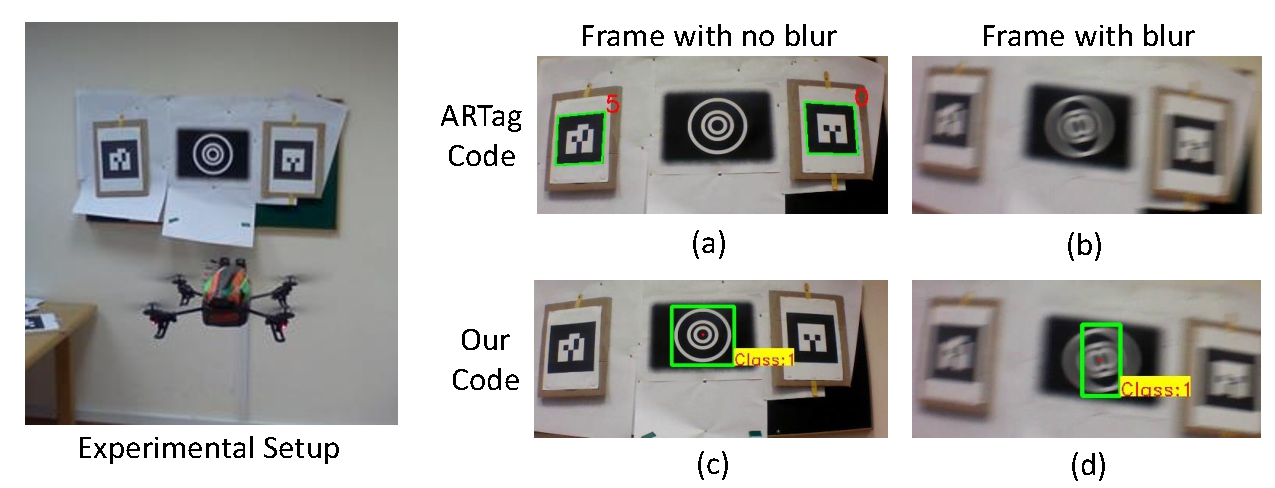
\includegraphics[width=\linewidth]{figures/fiducial/teaser}
  \caption[Overview]{Experimental setup and comparison of fiducial-based
    algorithms. A green border signifies success. 
    \textbf{(Left)} A drone encounters three different fiducials. 
    \textbf{(Right, Top)} Output of ALVAR~\cite{alvar} under favorable and blurred
    circumstances. No green border is seen in (b) signifying failure.
    \textbf{(Right, Bottom)} Output of the proposed fiducial. Green
    border is seen in both (c) and (d).
    \label{fig:fiducial_teaser}}
  \end{figure}

\section{Design of Blur Resistant Fiducial}

We begin by first motivating the need for a new blur resistant
fiducial by examining the performance of prior fiducials under motion
blur.  After this, we detail our design as well as the detection
algorithm used to find the fiducial in an image, or a video sequence.

\subsection{Prior Fiducials Under Motion Blur}\label{sec:blurtest}

Here we examine the performance of two popular fiducials under
motion blur.  Specifically we examine ARTags ~\cite{Fiala05} and
PiTags~\cite{Pitag13} given their differences in geometric design and
the availability of an API to develop applications to recognize the tags.
\footnote{RUNE-tag~\cite{runetag11} currently does not
provide access to an implementation to generate or recognize its tags. 
The circular data matrix~\cite{NaimarkF02} is available as a
commercial product, however it requires proprietary hardware.}

%To evaluate the ARTag and PiTag under blur, 
For controlled study, we simulate the appearance of the ARTag and PiTag
markers by scaling the tags to 150$\times$150 pixels.
Both fiducials are then blurred using linear motion blur at various
orientations with different  blur scales. The blur motion ranged from 15 to 50
in magnitude (measured in pixels), representing small to significant motion
blur. Figure~\ref{fig:artag_pitag} shows the visual appearance of the blurred
tags. We then try to detect the markers using the ALVAR library~\cite{alvar} and
PiTag library~\cite{ros_pitag}. The table in %the right side of
Figure~\ref{fig:artag_pitag} shows the recognition rate (in
percentage) of the two fiducials at various blur scales over all  orientations.
As we can see, the PiTag performance quickly diminishes under small amounts of
blur, while at 35 units, the ARTag's recognition rate drops to less than
20\%.

\begin{figure}[t!]
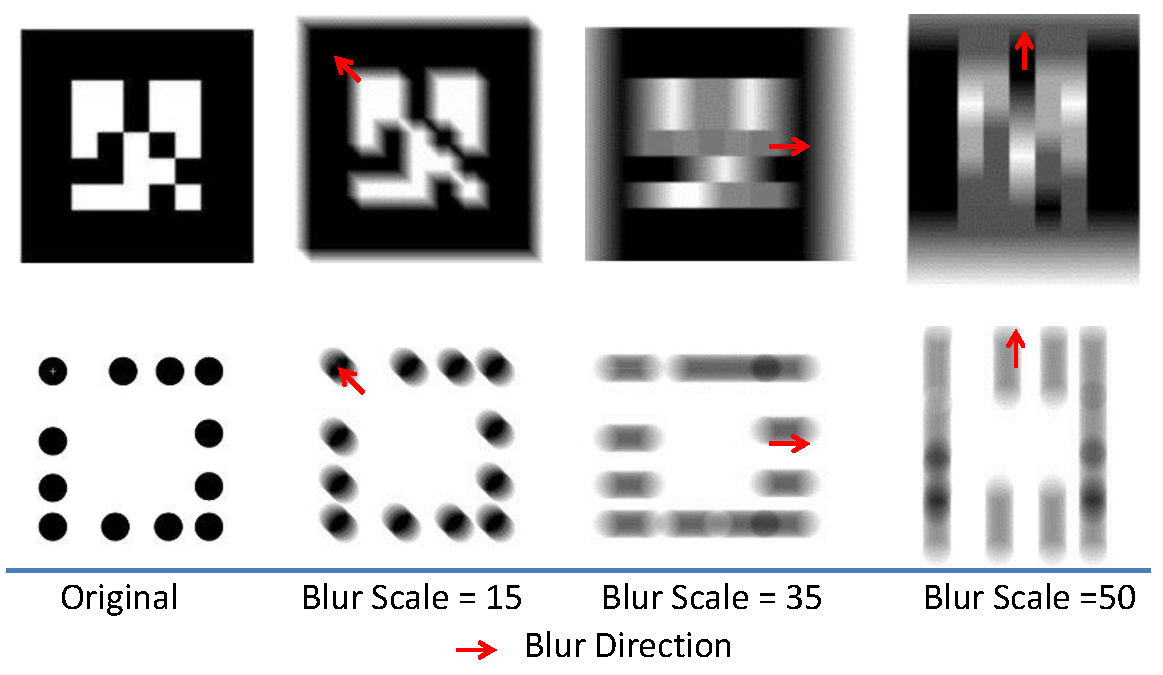
\includegraphics[width=\linewidth]{figures/fiducial/artag_pitag.pdf}
%\captionof{figure}{Blurred ARTag and Pi--tag with various blur scales}
%\captionof{table}{Recognition rate of ARTag and Pi-tag fiducial at various blur scales}

\begin{tabularx}{\linewidth}{|Y|Y|Y|}
\cline{1-3}
\small{Blur} & \multicolumn{2}{c|}{ \small{Recognition Rate}}
\\\cline{2-3}
\small{Scale}& \small{PiTag} &	\small{ARTag} \\ \cline{1-3}
\small{15} & \small{100} & \small{100} \\ %\cline{1-3}
\small{30} & \small{0} & \small{100} \\  %\cline{1-3}
\small{35} & \small{0} & \small{19} \\ %\cline{1-3}
\small{50} & \small{0} & \small{0} \\ \cline{1-3}
\end{tabularx}
\captionof{figure}[Comparison with PiTag and ARTag]{\textbf{Top:} The PiTag and
ARTag fiducials blurred with various blur scales at different orientations. \textbf{Bottom
    Table:} Recognition rate (in percent). We see that the recognition
  rates for both the tags are significantly reduced. For severe blur,
  detection fails.}
\label{fig:artag_pitag}
\end{figure}

\subsection{Blur Resistant Fiducial}

We propose a binary coded fiducial that uses concentric white rings of
equal widths on a black background with a blurred
border\footnote{Obviously, this design can be inverted to have a white
  background with black rings.}. The outermost and innermost rings
represent the start and end of the code and is embedded in the
fiducial.  The binary code is represented by the presence (or absence)
of rings between ``marker'' rings.

\begin{figure}
\centering
  
\includegraphics[width=.24\linewidth]{figures/fiducial/newconcentric_00.pdf}
  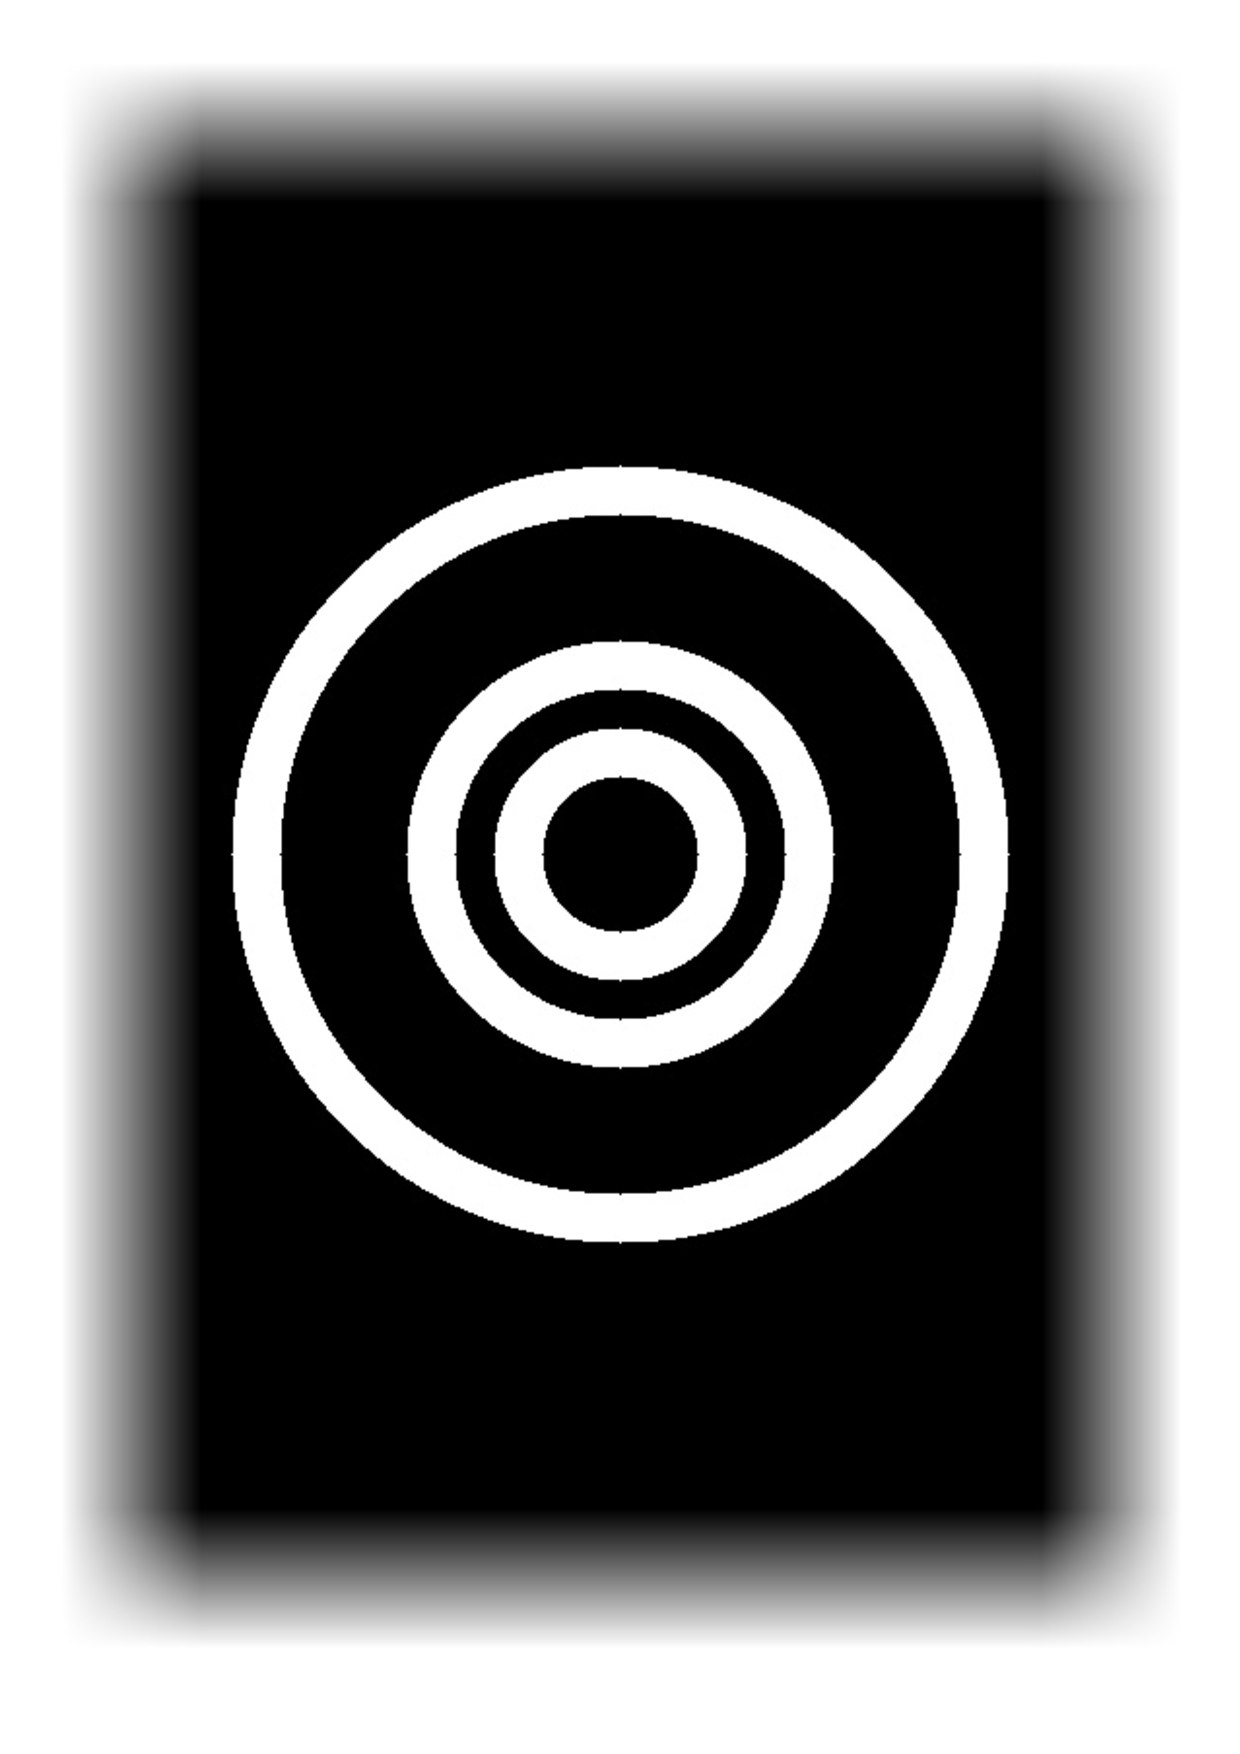
\includegraphics[width=.24\linewidth]{figures/fiducial/newconcentric_01.pdf}
  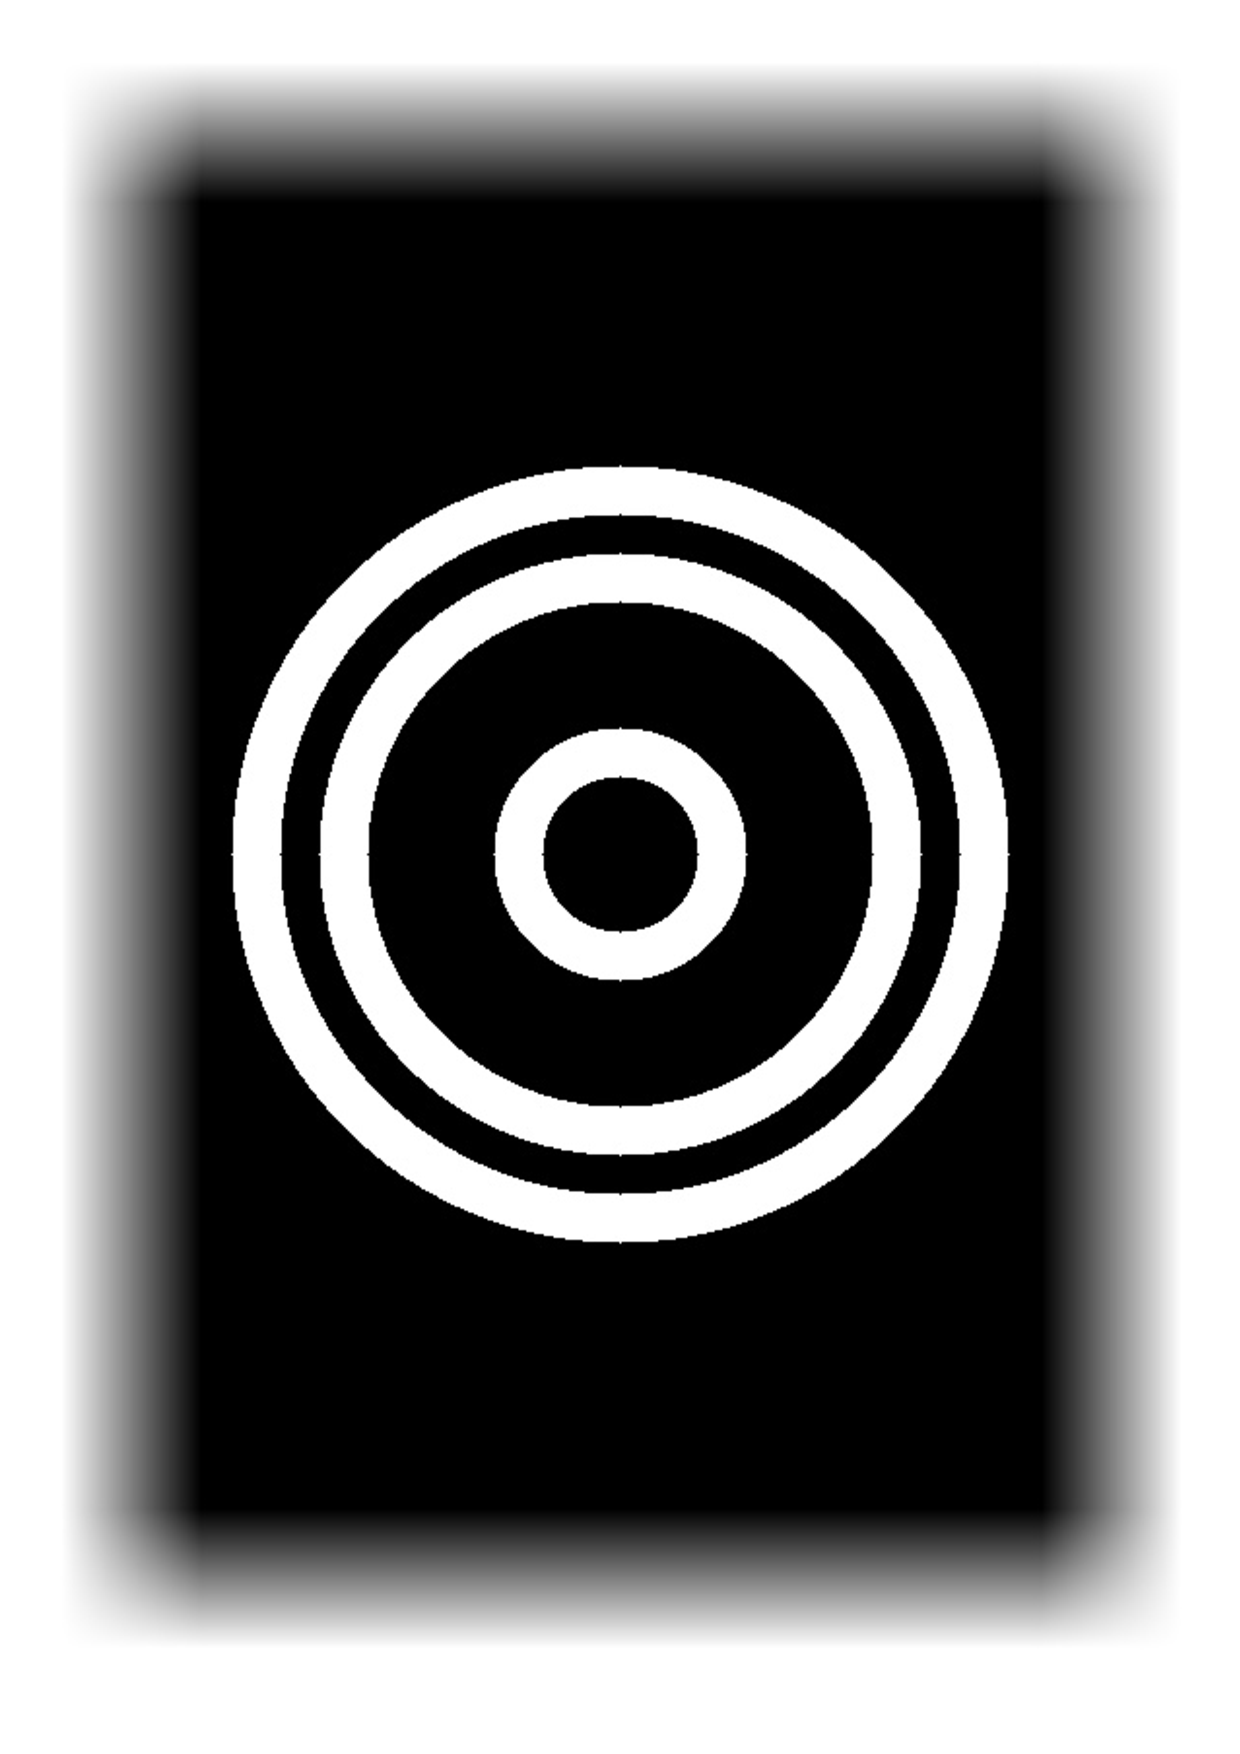
\includegraphics[width=.24\linewidth]{figures/fiducial/newconcentric_10.pdf}
  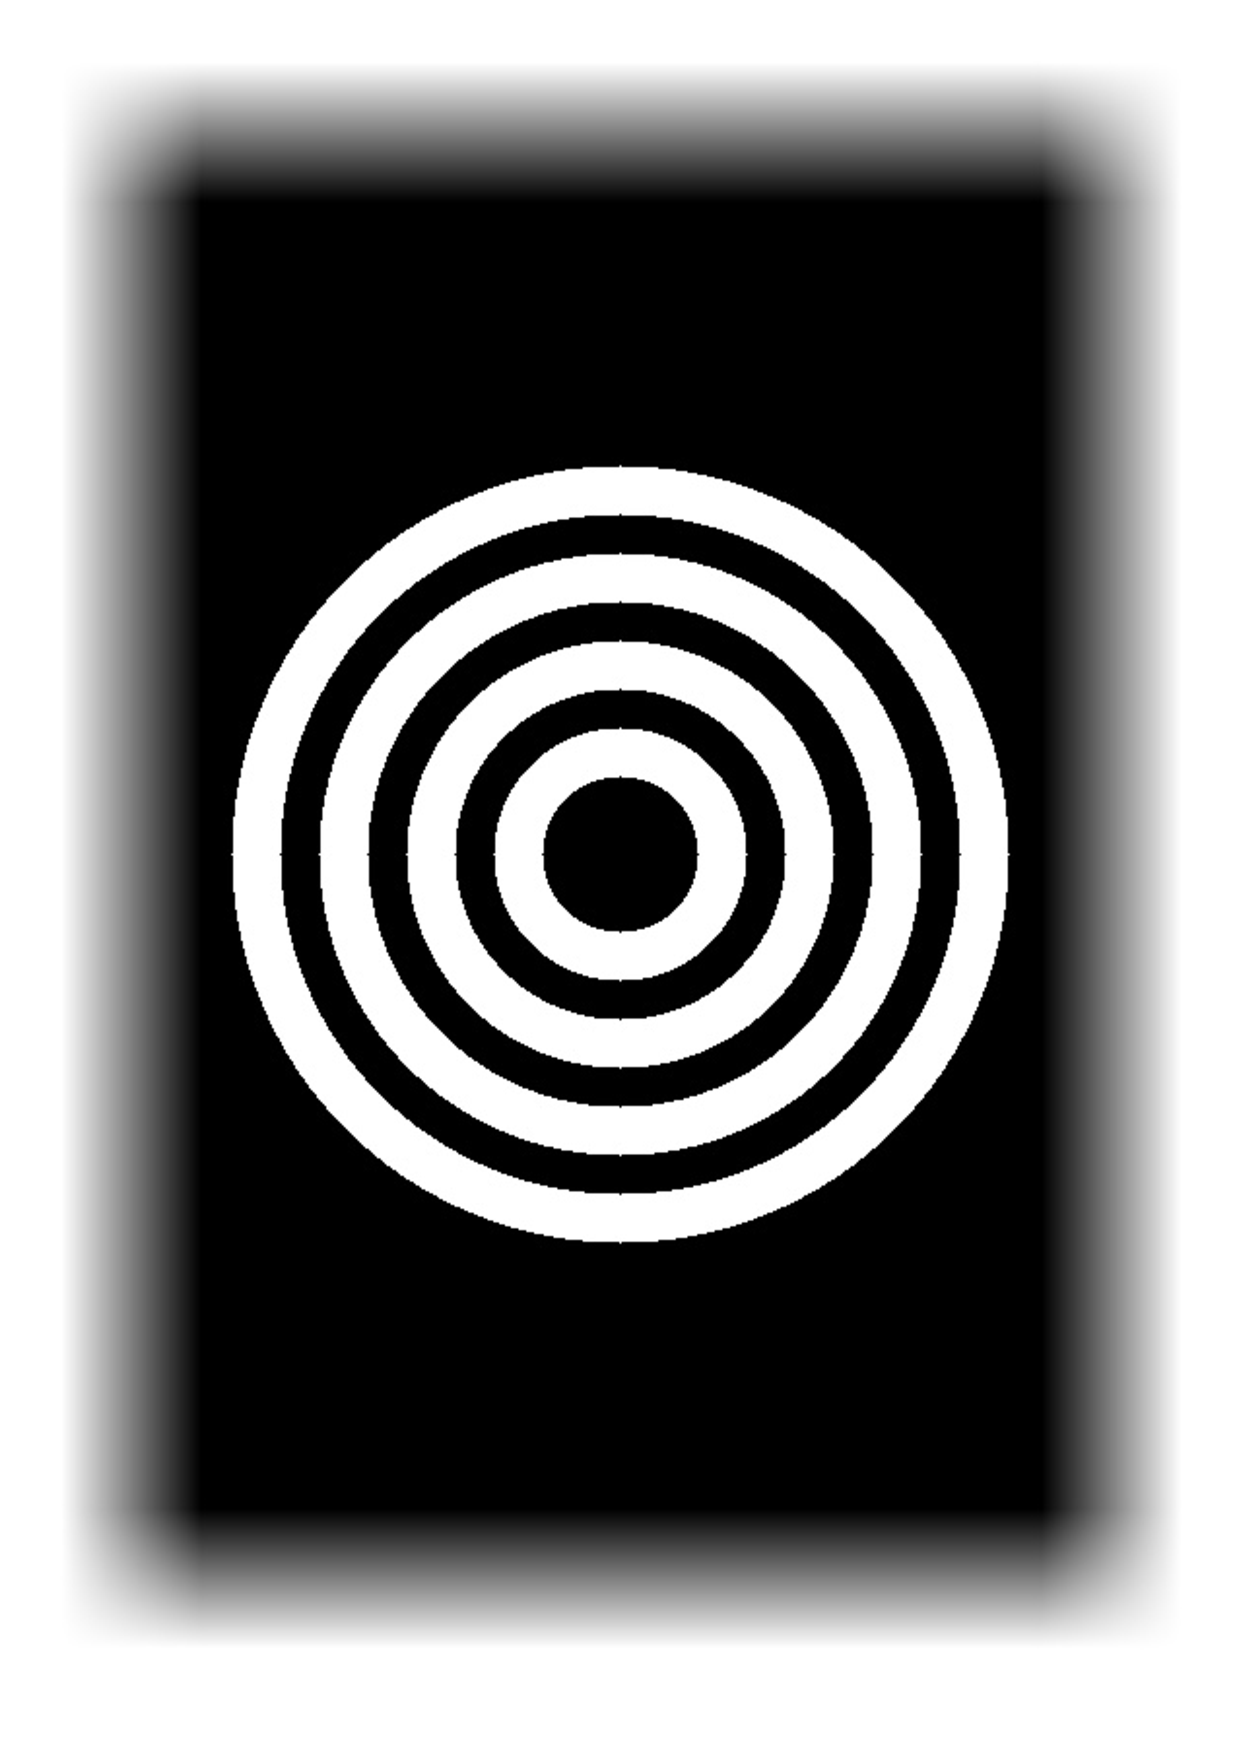
\includegraphics[width=.24\linewidth]{figures/fiducial/newconcentric_11.pdf}
  \caption[Two bit, binary  fiducials]{Two bit, binary  fiducials, representing,
  from left to right 00, 01, 10, and 11.}
  \label{fig:fiducials}
\end{figure}

Depending on which ring is present or absent, the resulting binary
code will change. The number of different patterns depends on the
number of bits in the binary code. For example, if the binary code has
three bits, there will be a maximum of three rings between marker
rings and we end up with eight different patterns.
Figure~\ref{fig:fiducials} shows two bit binary fiducials.


Our fiducial detection strategy is different from
\cite{NaimarkF02,Pitag13} and works under significant amounts of blur.
As previously mentioned, our approach works under the observation that
the motion blur for the quadcopter's camera can be well modeled as
linear motion.  This linear motion blur assumption has been shown to
be reasonable in prior works~\cite{Moshe:2003,Moshe:2004}
targeting camera motion blur. Under this assumption, the scene
content perpendicular to the blur direction is unaffected by the blur.
Because of our circular design, the direction perpendicular to the
linear motion will still be recognizable as a linear pattern.
Figure~\ref{fig:blur_direction} shows examples of this using a pattern
under 
various motion directions.

\begin{figure}[h!]
\centering
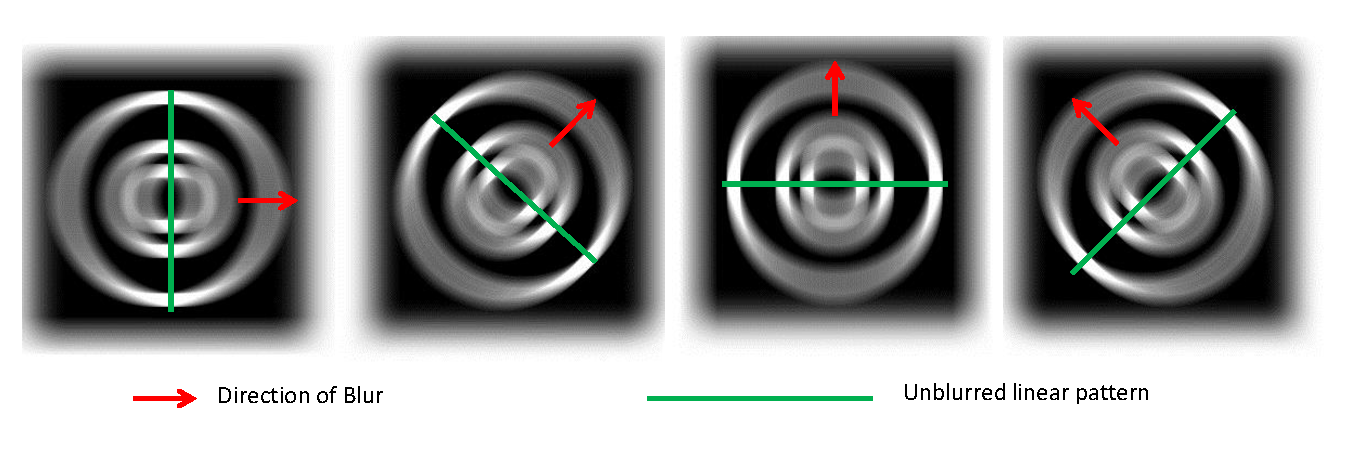
\includegraphics[width=\linewidth]{figures/fiducial/blur_direction}
\caption{Change in blur direction changes the location and orientation
  of an unblurred linear pattern.}
\label{fig:blur_direction}
\end{figure}


\subsection{Detection Algorithm}

Figure~\ref{fig:overall_flow} shows the process involved in fiducial
detection. We give a brief overview of our algorithm here with each
step described in detail afterwards.  Our detection algorithm has four
steps. In Step~1, we apply a Gabor filter on the image to isolate the
potential locations of the pattern.  In Step~2, we find clusters of
patches in the Gabor output.  In Step~3, we perform Principal
Component Analysis (PCA) on each cluster to find the dominant
direction unaffected by blur.  Finally in Step~4, based on the
direction detected, we extract the intensity profile of the pattern
and classify the fiducial. 

\begin{figure*}[ht!]
  \centering
  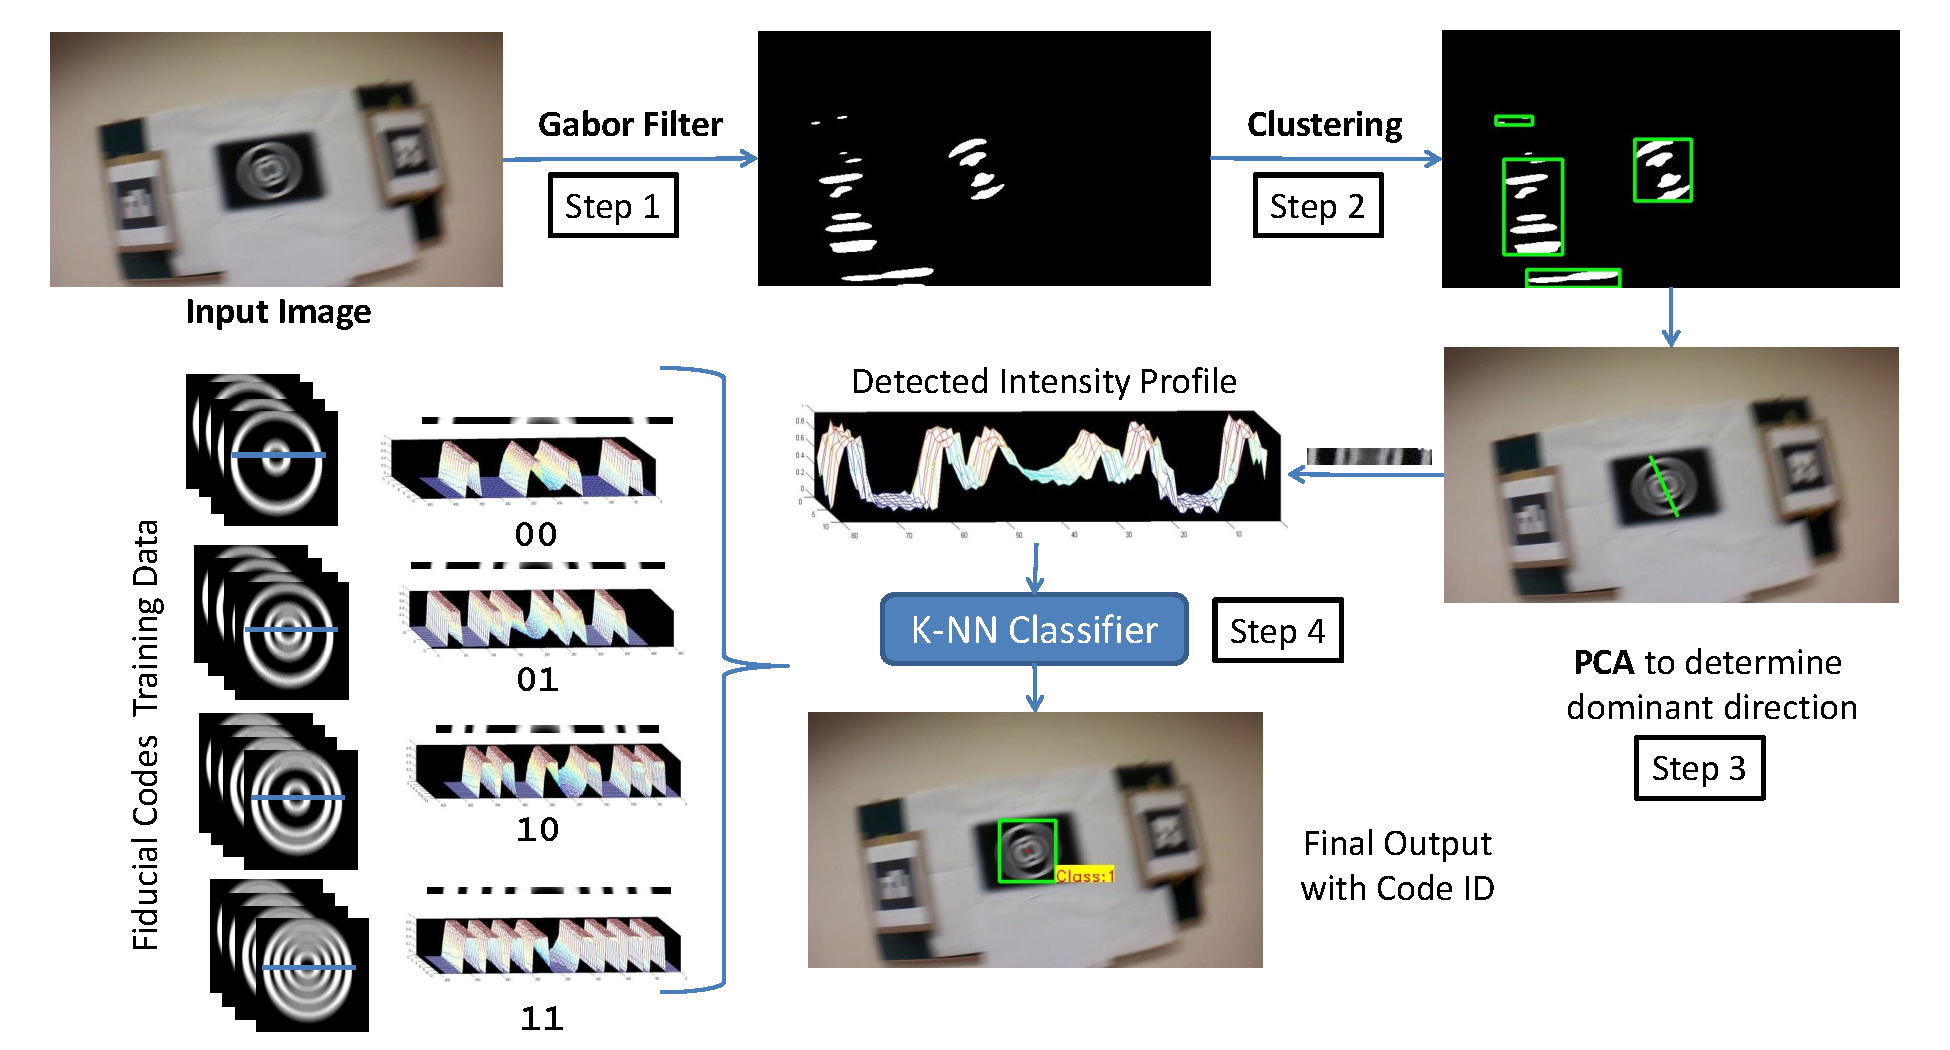
\includegraphics[width=0.8\linewidth]{figures/fiducial/overall_flow.pdf}
  \caption[Overall Workflow]{An overview of our algorithm.
    The four step process includes (Step 1) Filtering,
    (Step 2) Component clustering, (Step 3) Dominant direction determination
    and (Step 4) Classification using prior training data.}
  \label{fig:overall_flow}
\end{figure*}

%\noindent Details of each of the steps are as follows:\\
\textbf{Gabor filter:}~~A 2D Gabor filter is a Gaussian kernel function
modulated by a sinusoidal plane wave~\cite{Kruizinga:2002}. It is used to find
high gradient patches. In our case, it is used to detect portions
of the circular fiducials that were not affected by the blur.
We applied the Gabor filter in eight
different orientations ($\theta = 0, 45, 90, \ldots, 225, 270, 315$).  The
following parameters were used for creating each Gabor kernel: $\lambda$ (wavelength) $= 8$, $\gamma$
(aspect ratio) $= 0.5$, $\sigma$ (spread) $= 0.56\lambda$, $\psi$
(phase angle) $= 0$ (for real part), $\pi/2$ (for imaginary part).
Then $\ell^2$-norm of outputs along all orientations is calculated and finally
$\ell^2$-normalized image is thresholded with threshold set to $0.4$ (on scale of zero to
one).  For further details to the Gabor filter, see~\cite{Kruizinga:2002}.
%% MBS - is the Kruizinga filter reasonable to cite?

\textbf{Clustering:}~~The binarized Gabor filter responses are
treated as a set of connected components in the image.   Clustering
is used to find components that are located in a close spatial region.  We do
this via hierarchical clustering~\cite{ALGLIB} using unweighted
average linkage with a distance threshold set to 150.

\textbf{PCA:}~~For each clustered set of components, we apply
PCA to determine the dominant direction.  This is done by examining
the orientation of the first principal component.  We then extract an
intensity profile patch in the input image along this direction as it
extends through the bounding box of the cluster. The signature of this
profile will be used to identify the code.

After finding the intensity profile, we project the pixel intensities,
and record the number and width of the white-to-black transitions.  If
the number of transitions, or the width of the transitions is not
consistent with what is allowable by our code, we reject the clustered
region as a potential fiducial.  Clustered components that have
allowable transitions counts and transitions with uniform widths are
further considered for classification to determine the binary code.

\textbf{Classification:}~~As mentioned above, a small image patch
containing the intensity profile of the fiducial is used to identify
which of the many fiducials might be present and is represented by a
code.  We found that a training-based method using the k nearest
neighbor (k-NN) technique gave better results than trying to find
binary code directly by determining the presence (or absence) of ring
at particular positions in the image patch. This required
training-data which was easy to generate. A synthetic fiducial
is blurred along 36 orientations (0, 10, 20, \ldots , 350) with blur
scale set to 40, and the intensity profile along the first principal
component from every output is taken as training data for that
fiducial. Figure~\ref{fig:training_data} shows the process of
creating training data for fiducial with binary code ``01'' embedded
in it.  For a query image patch, we normalize the intensity range, and
then compare this information against the training data. The class
label from the closest top $K=5$ images in the training data is used
to label the patch.

\begin{figure}[h!]
\centering
  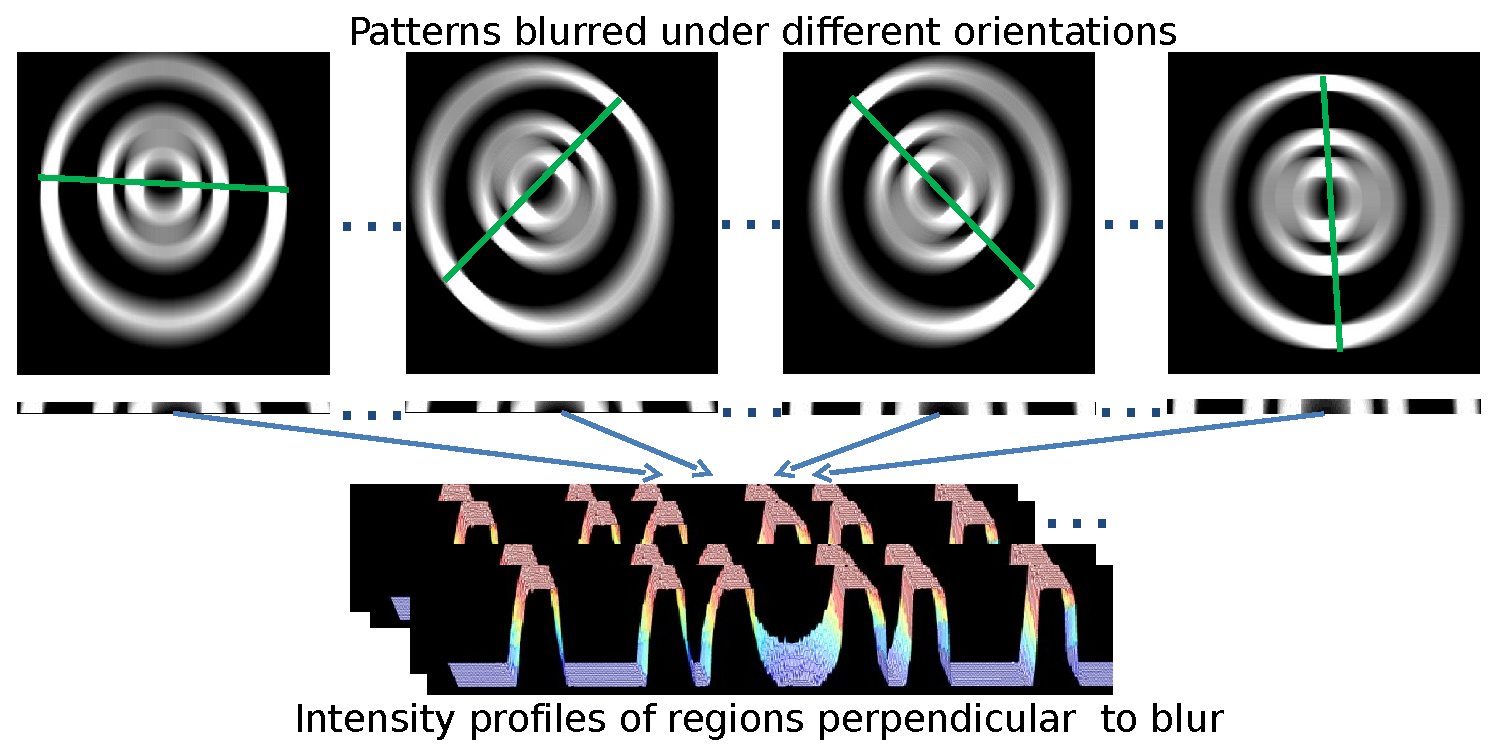
\includegraphics[width=0.95\linewidth]{figures/fiducial/training_data.pdf}
  \caption[Creation of training data for classification  for the fiducial with
  binary code ``01'']{Creating training data for the fiducial with binary code
  ``01'': The synthetic pattern is blurred along various orientations and the
  intensity profile monitored and stored. The same process is used to create
  training data for all other fiducials.}
  \label{fig:training_data}
\end{figure}

\begin{comment}
We are able to find the number of rings in the fiducial by finding
number of transitions in the intensity profile. To increase the classification
accuracy, training data for patterns having same number of rings are grouped together; e.g., in two bit
binary coded fiducial, training data for pattern ``01'' and ``10'' will be
grouped together. In three bit binary coded fiducial, training data for pattern
``001'', ``010'' and ``100'' will form one group, while training data for
pattern ``110'', ``011'' and ``101'' will be in other group, and so on.
Depending on the number of detected rings in test pattern, it is matched
against corresponding group in the training data, again using  the K-NN.
If we detect either zero rings or maximum possible
rings in the test pattern, there will be no need to do further classification, we
can classify the pattern as class 0 or the maximum class containing all 1s.
\end{comment}

\section{Experimental Validation}

We have implemented our algorithm in C++ using the OpenCV library.
Experiments were performed on a laptop with Intel Core i7
processor(@3.4GHz) and 4GB RAM. (Please check our webpage
\url{http://meghshyam.github.io/fiducial/} for details of source code
and all datasets)
%Video clips of collected data are provided in the supplementary
%material.
% Meghshyam: Is it a desktop PC or a laptop?

Our system has been tested on several image sequences captured from an
AR Drone quadcopter.  The drone was flown indoors looking at patterns
attached to various walls. Each image sequence contains frames of
different fiducials. Some sample outputs for each fiducial
is shown in Figure~\ref{fig:out_outputs}. Our detection process takes
around 0.3 seconds which translates to slightly over three frames per
second.


\begin{figure}[h!]
\centering
  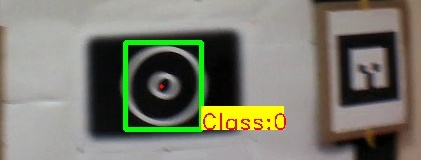
\includegraphics[width=0.4\linewidth]{figures/fiducial/output_00.jpg}
  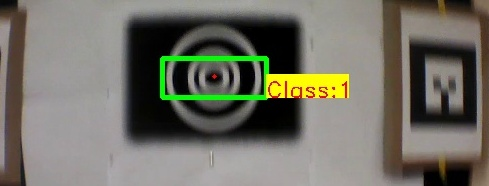
\includegraphics[width=0.4\linewidth]{figures/fiducial/output_01.jpg}

  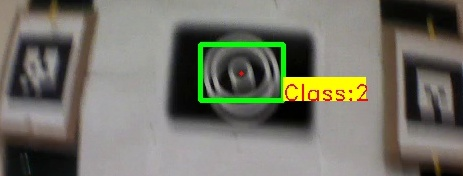
\includegraphics[width=0.4\linewidth]{figures/fiducial/output_10.jpg}
  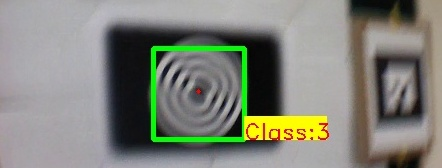
\includegraphics[width=0.4\linewidth]{figures/fiducial/output_11.jpg}
  \caption[Output of our fiducial detection algorithm]{Output of our fiducial
  detection algorithm on sample images. The class label shown is the decimal
  equivalent of the binary coded fiducial.}
  \label{fig:out_outputs}
\end{figure}

Our system has also been tested on images containing multiple fiducial
patterns in the same frame. Our algorithm successfully detected
all fiducials as well as correctly classified them as shown in
Figure \ref{fig:output_all}.

\begin{figure}[ht!]
\centering
  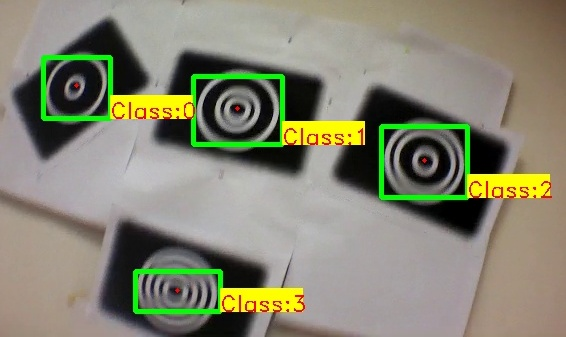
\includegraphics[width=.45\linewidth]{figures/fiducial/output_all_2.jpg}
  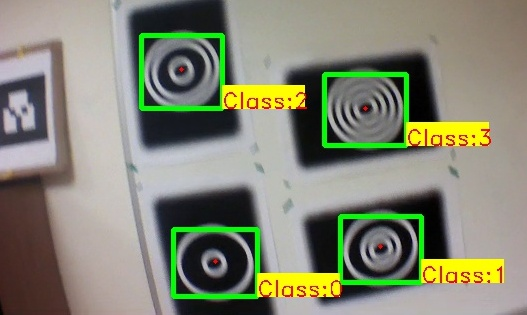
\includegraphics[width=.45\linewidth]{figures/fiducial/output_test_all1.jpg}
  \caption[Result: Multiple Fiducials Detection]{Multiple fiducials in the same
  frame can be efficiently detected. }
  \label{fig:output_all}
\end{figure}

%\subsection{Comparisons}

We compare our results with the commonly used ARTag. We also compare
our results with Blur-driven tracker (BLUT)\cite{Wu:2011}.

\subsection{Comparison with ARTag}
First, we repeat the same blur simulation experiment
(Section~\ref{sec:blurtest}) on the proposed fiducial. Specifically,
we build our blur resistant patterns at 150$\times$150 pixel
resolution and blurred them along various orientations with different
blur scales. 
%Then, we tried to detect our fiducial using a 2-bit
%patterns using algorithm presented in earlier section.

\begin{figure}[t!]
  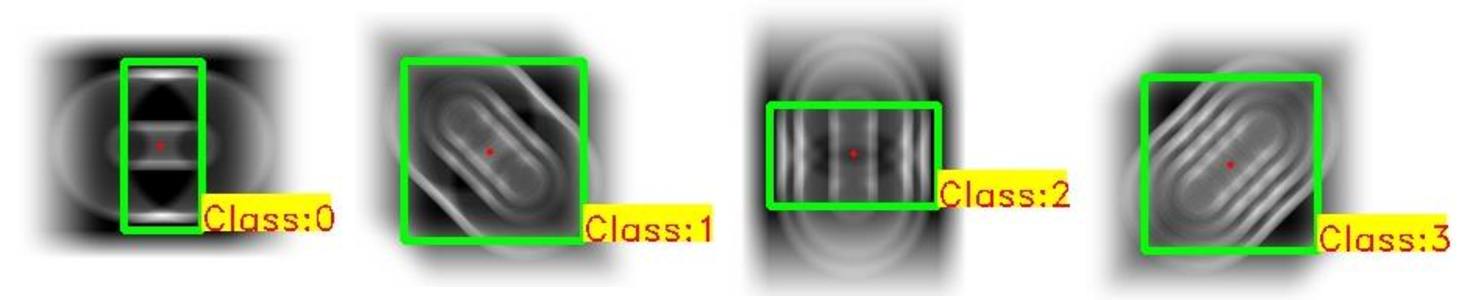
\includegraphics[width=\linewidth]{figures/fiducial/blur_maximum.pdf}
  \caption[Result: Synthetic experiment]{On synthetic experiments, we increase
  the blur much beyond the best possible results (see Figure~\ref{fig:artag_pitag}) for
    prior methods. Even upto 65 units, the algorithm is successful.}
  \label{fig:blur_maximum}
\end{figure}

Qualitatively, we see in Figure~\ref{fig:blur_maximum} that despite of
even more blur than earlier described (50 units or more), detection is
still feasible and practical.  Quantitatively, the comparison of
recognition rate is shown in Figure~\ref{fig:recognition_rate}.
Even under more severe blur, of 65 pixels, the algorithm is
successful.  Our recognition is 100\% for all codes except the ``00''
which is undetectable after 50 pixels blur (which is still
significantly better than ARTag).  Reasons for the lower performance
when``00'' tags are present, is discussed in
Section~\ref{sec:discussion}.

\begin{figure}[h!]
\centering
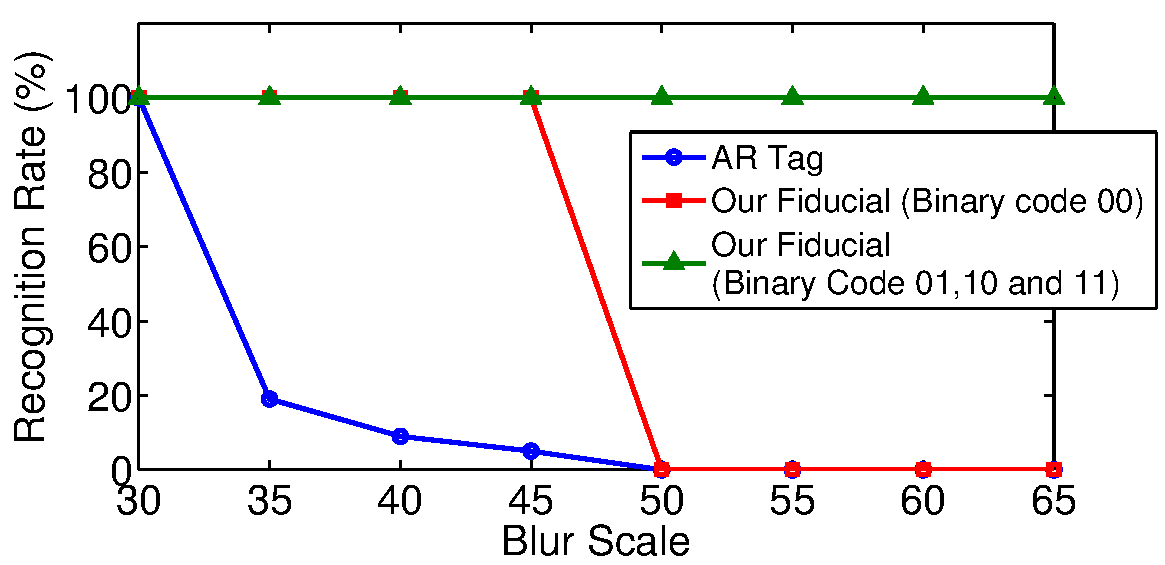
\includegraphics[width=\linewidth]{figures/fiducial/recognition_rate.pdf}  
\caption[Comparison of recognition rate of fiducials]{Comparison of recognition
rate of fiducials.  The proposed fiducial handsomely outperforms prior methods.}
\label{fig:recognition_rate}
\end{figure}


We also performed analysis to detect how accurately the center of the
blur pattern can be localized under blur.  To do this, we have
simulated data along different blur orientations for all patterns over
eight different blur scales (30 to 65 with step size of 5). Values for
the localization of the pattern ``00'' after blur with 50 pixels is
omitted since the pattern cannot be detected. From
Table~\ref{tab:blur_angle_center}, it can be clearly seen that the 
mean error in locating center by our algorithm is within approximate 3
pixels, or 3\% of the diameter of fiducial.

\begin{table}[h!]
  \centering
  \begin{tabularx}{0.6\linewidth}{|Y|Y|}
    \cline{1-2}
    \footnotesize{Blur} & \footnotesize{Mean($\pm$std) error}  \\
    \footnotesize{angle} & \footnotesize{(in pixels)}  \\
    \cline{1-2}
    \footnotesize{0} & \footnotesize{1.33 $\pm$ 0.40}  \\
    \footnotesize{22} & \footnotesize{2.42 $\pm$ 1.05} \\
    \footnotesize{45} & \footnotesize{1.46 $\pm$ 0.65}  \\
    \footnotesize{67} & \footnotesize{2.39 $\pm$ 1.28}  \\
    \footnotesize{90} & \footnotesize{1.83 $\pm$ 0.25}  \\
    \cline{1-2}
  \end{tabularx}
    \caption{Center localization error.
      Error is computed for various blur angles over various scales.}
    \label{tab:blur_angle_center}
\end{table}



\begin{comment}
\begin{figure*}
\centering
\begin{tabular}{c|c}
\begin{subfigure}[b]{0.45\linewidth}
\centering
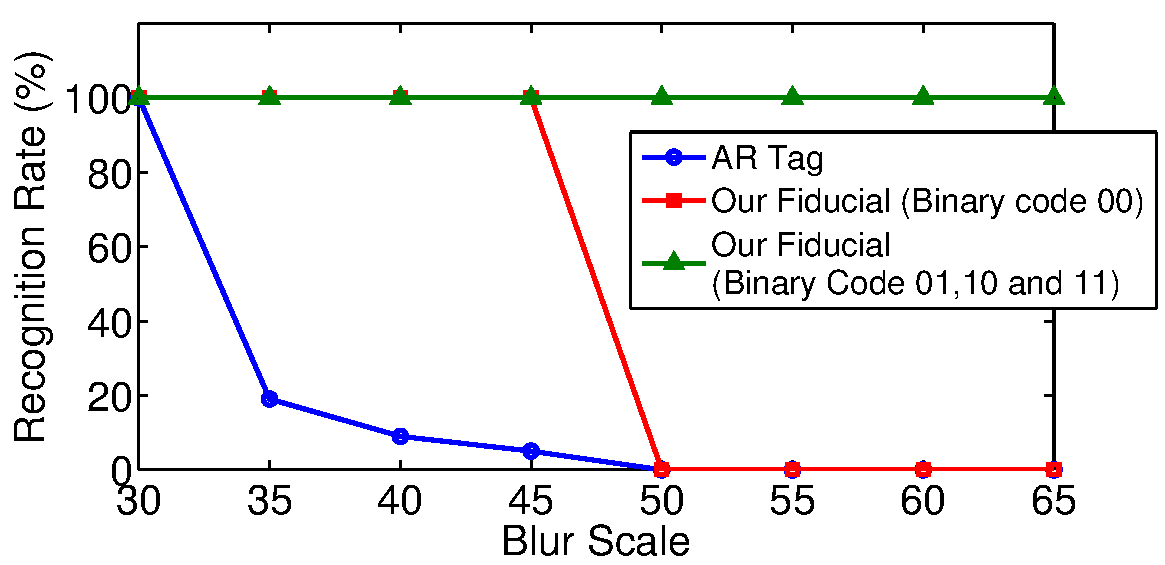
\includegraphics[width=\linewidth]{figures/fiducial/recognition_rate.pdf}
\caption{Comparison of recognition rate of fiducials}
\label{fig:recognition_rate}
\end{subfigure}
&
\begin{subfigure}[b]{0.25\linewidth}
\centering
\begin{tabularx}{\textwidth}{|c|Y|}
\cline{1-2}
\footnotesize{Blur} & \footnotesize{Mean($\pm$std) error}  \\
\footnotesize{angle} & \footnotesize{(in pixels)}  \\
\cline{1-2}
\footnotesize{0} & \footnotesize{1.33 $\pm$ 0.40}  \\
\footnotesize{22} & \footnotesize{2.42 $\pm$ 1.05} \\
\footnotesize{45} & \footnotesize{1.46 $\pm$ 0.65}  \\
\footnotesize{67} & \footnotesize{2.39 $\pm$ 1.28}  \\
\footnotesize{90} & \footnotesize{1.83 $\pm$ 0.25}  \\
\cline{1-2}
\end{tabularx}
\caption{Center localization error}
\label{tab:blur_angle_center}
\end{subfigure}
\end{tabular}
\caption{(a): Comparison of recognition rate of the ARTag and our fiducials on
blur simulated data at various blur scales. It can be seen that except for the
fiducial with binary code ``00'', our fiducials are recognized all times.
(b): Table showing the mean error and standard deviation of the localized fiducial center
versus the ground truth.  Error is computed for various blur angles over
different blur scales.}
\label{fig:simulated_blur}
\end{figure*}
\end{comment}

\subsection{Real Data}

We also compared results on the recorded feed using the AR Drone
quadcopter. In our experimental setup, we have placed two ARTags in
the scene along with our fiducial to compare the resilience of blur by
each fiducial type. We have used ar\_track\_alvar, ROS Wrapper for the
ALVAR library~\cite{ros_alvar}, to detect the ARTags from the stream
captured with the quadcopter camera. In each test dataset, we have
used different two bit binary coded fiducial and recorded video of
around two minute duration (i.e., around 1000 frames).  The quadcopter
was flown in a routine manner in the room with its camera facing the
wall. The comparison of the recognition
rate is shown in Table~\ref{tab:recognition_accuracy}. Recognition
rate of our fiducials ranges from 86.5\% to 94.1\%, while the ARTag is
60.3\% to 65.6\%.  Classification accuracy of all fiducials (ARTag as
well as ours) was approximately 100\%, i.e., when tags were detected
they were the correct fiducials and not other objects in the scene.

\begin{table}[t!]
  \centering
  \begin{tabularx}{\linewidth}{|c|Y|Y|Y|Y|}
    \cline{1-5}
    \multirow{2}{*}{Test \#} & {Number}
    &{Binary} &\multicolumn{2}{c|}{Recognition Rate (\%)} \\
    \cline{4-5} & {of frames}& {Code}& ARTag & Our Fiducial \\\cline{1-5}
    1 & 1205 & 00 &  65.6 & 86.5  \\ \cline{1-5}
    2 & 1047 & 01 &  61.9 & 94.1  \\ \cline{1-5}
    3 & 1102 & 10 &  62.4 & 92.74 \\ \cline{1-5}
    4 & 1081 & 11 &  60.3 & 93.54  \\ \cline{1-5}
  \end{tabularx}
  \caption[Comparison of Recognition Rate: Real Data]{ 
  \label{tab:recognition_accuracy} Recognition rate of ARTag and proposed fiducials on real
    data captured through AR Drone. Each row shows analysis of a test
    dataset captured for our fiducial with different binary codes embedded in it.
    Each dataset has around 1000 frames captured representing roughly two
    minutes of video.} 
\end{table}

In another setup we arranged our fiducials on four sides of a box and
revolved the quadcopter around the box (See  \cite{video}).
Later, we repeated the process by replacing our fiducial by ARTags. Figure~\ref{fig:setup} shows some
frames from this sequence as well as the performance of both
fiducials. The overall detection rate of our tags is 90\% while that
of ARTags is only around 60\%.

\begin{figure*}
\begin{subfigure}[b]{.19\textwidth}
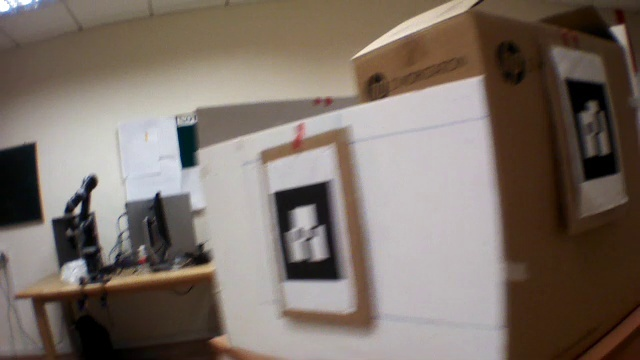
\includegraphics[width=\linewidth]{figures/fiducial/setup_artag/output_79.jpg}
\end{subfigure}
\begin{subfigure}[b]{.19\textwidth}
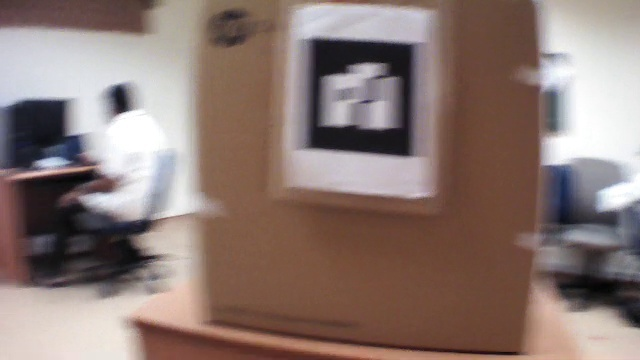
\includegraphics[width=\linewidth]{figures/fiducial/setup_artag/output_150.jpg}
\end{subfigure}
\begin{subfigure}[b]{.19\textwidth}
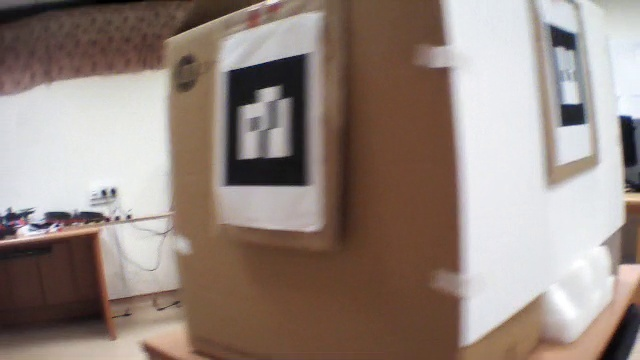
\includegraphics[width=\linewidth]{figures/fiducial/setup_artag/output_194.jpg}
\end{subfigure}
\begin{subfigure}[b]{.19\textwidth}
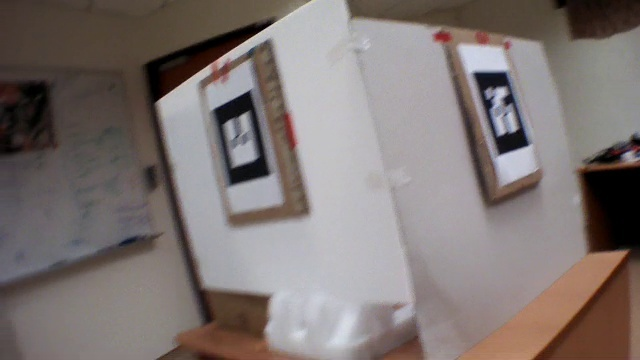
\includegraphics[width=\linewidth]{figures/fiducial/setup_artag/output_339.jpg}
\end{subfigure}
\begin{subfigure}[b]{.19\textwidth}
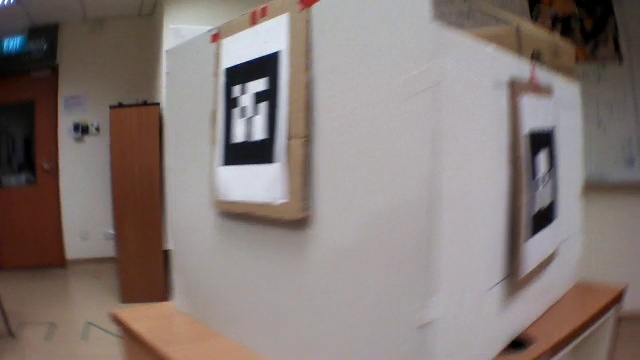
\includegraphics[width=\linewidth]{figures/fiducial/setup_artag/output_480.jpg}
\end{subfigure}\\
\begin{subfigure}[b]{.19\textwidth}
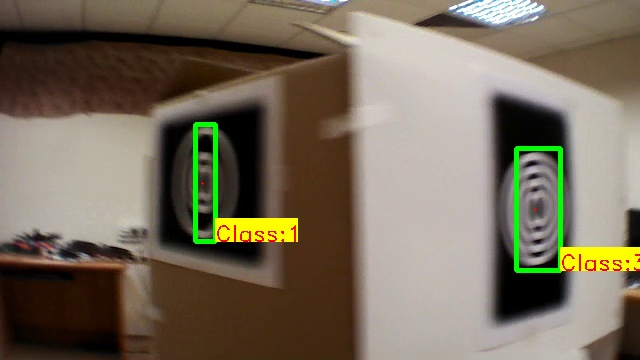
\includegraphics[width=\linewidth]{figures/fiducial/setup_our/output_6/output_514.jpg}
\end{subfigure}
\begin{subfigure}[b]{.19\textwidth}
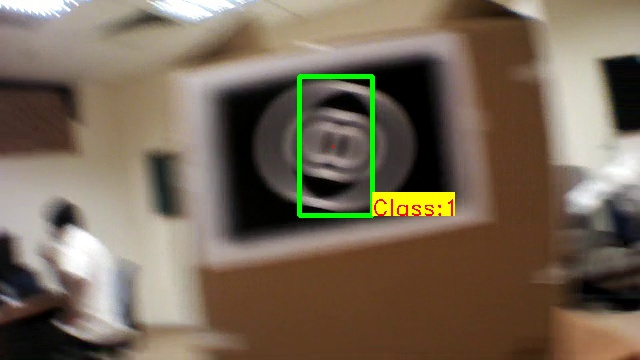
\includegraphics[width=\linewidth]{figures/fiducial/setup_our/output_2/output_64.jpg}
\end{subfigure}
\begin{subfigure}[b]{.19\textwidth}
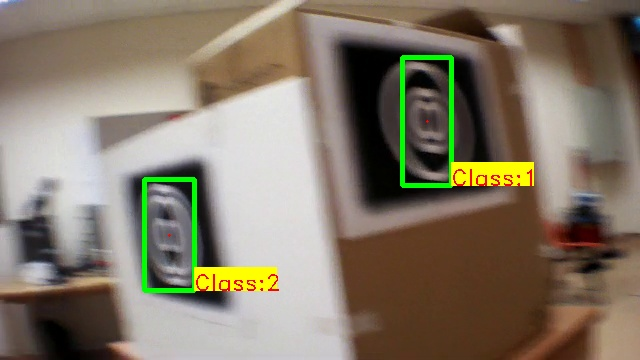
\includegraphics[width=\linewidth]{figures/fiducial/setup_our/output_2/output_35.jpg}
\end{subfigure}
\begin{subfigure}[b]{.19\textwidth}
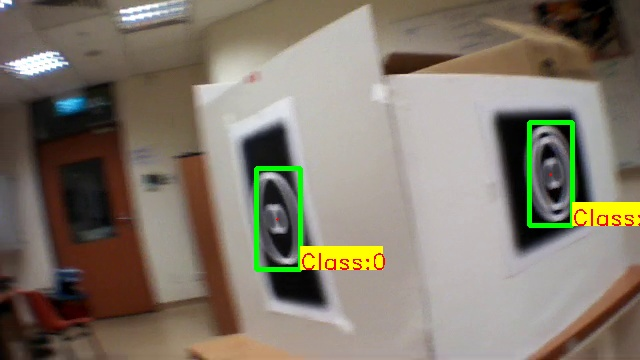
\includegraphics[width=\linewidth]{figures/fiducial/setup_our/output_2/output_330.jpg}
\end{subfigure}
\begin{subfigure}[b]{.19\textwidth}
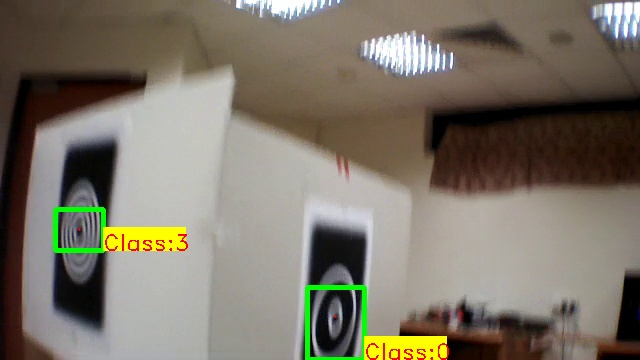
\includegraphics[width=\linewidth]{figures/fiducial/setup_our/output_6/output_943.jpg}
\end{subfigure}\\
\begin{subfigure}[b]{\textwidth}
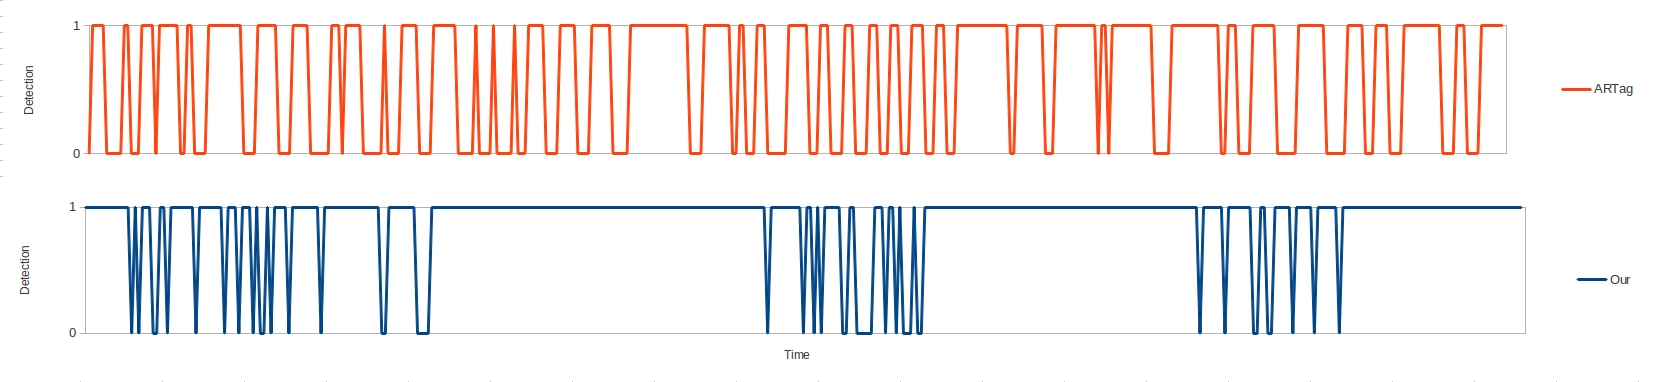
\includegraphics[width=\linewidth]{figures/fiducial/compare_detection.jpg}
\end{subfigure}
\caption[Comparison of ARTag and our fiducial when quadcopter is
  revolving around our setup]{Comparison of ARTag and our fiducial when quadcopter is
  revolving around our setup. 
\textbf{Top} ARTags are not detected, shown by an absence of green rectangles. \textbf{Middle} In
similar conditions, proposed fiducials are successfully
detected. Overall detection rate of proposed
fiducials is 90\% while that of ARTags is around 60\%. 
\textbf{Bottom Rows} Time view of detection. ARTag is ``choppy'' with
frequent losses, while the proposed fiducial (extreme bottom) is
``up'' almost all the 
time.}
\label{fig:setup}
\end{figure*}


\subsubsection{Comparison with BLUT}

We also compare our approach with tracking designed for blurred input
scenes.  We have used four image sequences (consisting of around 1000
frames each). Each sequence contains different fiducials so that we
are able to contrast the performance of BLUT~\cite{Wu:2011} with the
proposed method.  From the images in the top rows of
Figure~\ref{fig:BLUT_compare_00} and Figure~\ref{fig:BLUT_compare_01},
we can see that BLUT is able to track the fiducial when the position
of fiducial does not change too much in successive frames. Also, it
can be seen that once BLUT loses track of the fiducial, it is not
able to recover. Since our approach detects the code in each frame,
large changes in the pattern's position is not an issue.  Some of our
detection results are also shown in Figure~\ref{fig:BLUT_compare_00}
and Figure~\ref{fig:BLUT_compare_01}.

We have also found that even if we reset the BLUT tracker after it
loses track, the tracker will once again malfunction after around 100
frames (approximately within 6 seconds). When we checked the timestamp
data from image header captured through the AR Drone, we found that,
there was a difference of 0.14 seconds between two successive frames
indicating the dropping of video frame (normal 30fps should have a gap
of 0.033 seconds). Also, there were around 50 instances in 1000 frames
where the timestamp difference between two successive frames was
greater than 0.1 seconds. As such, it appears one of the main culprits
causing the BLUT tracker to fail is the dropping of frames combined
with the unstable motion of quadcopter, resulting in large discrepancies in
the  position of the fiducial between successive frames.

\begin{figure*}
\begin{subfigure}[b]{.19\textwidth}
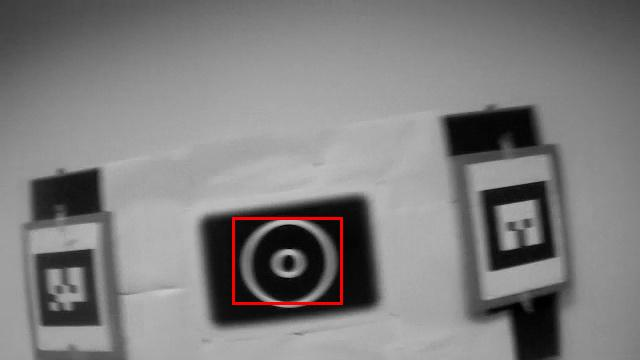
\includegraphics[width=\linewidth]{figures/fiducial/BLUT_output_00/2.jpg}
\end{subfigure}
\begin{subfigure}[b]{.19\textwidth}
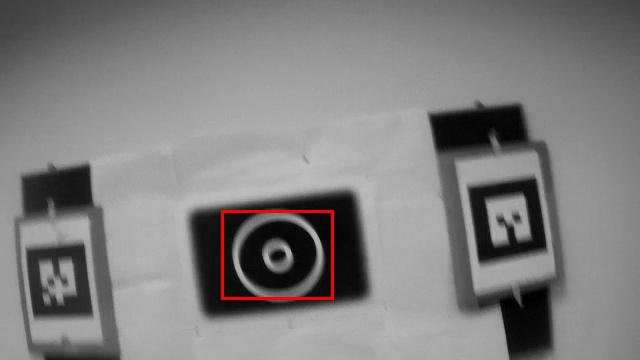
\includegraphics[width=\linewidth]{figures/fiducial/BLUT_output_00/3.jpg}
\end{subfigure}
\begin{subfigure}[b]{.19\textwidth}
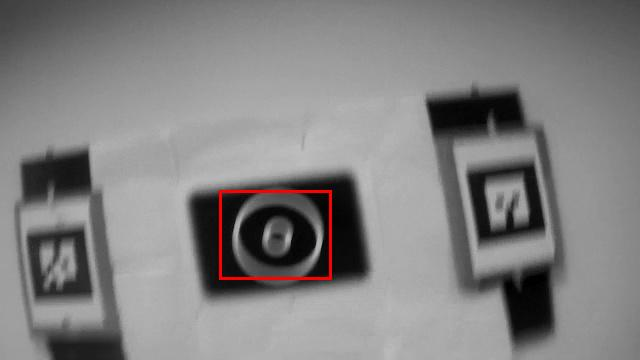
\includegraphics[width=\linewidth]{figures/fiducial/BLUT_output_00/4.jpg}
\end{subfigure}
\begin{subfigure}[b]{.19\textwidth}
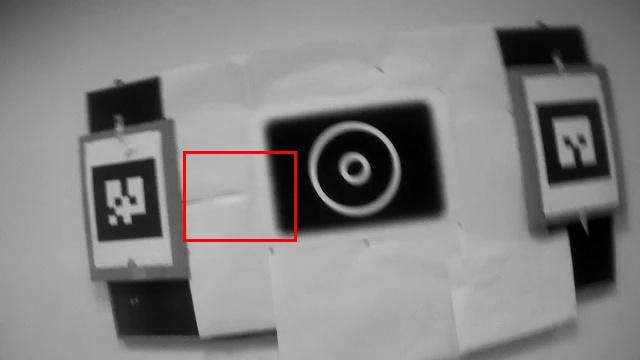
\includegraphics[width=\linewidth]{figures/fiducial/BLUT_output_00/5.jpg}
\end{subfigure}
\begin{subfigure}[b]{.19\textwidth}
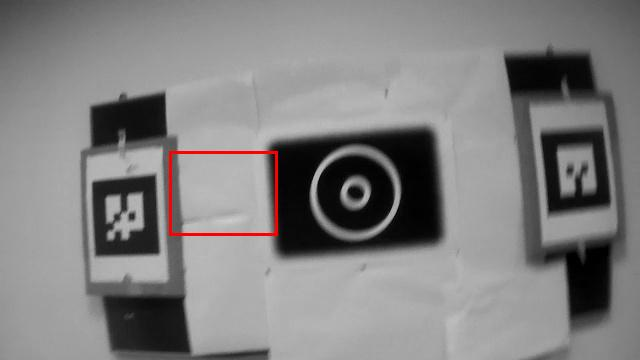
\includegraphics[width=\linewidth]{figures/fiducial/BLUT_output_00/6.jpg}
\end{subfigure}\\
\begin{subfigure}[b]{.19\textwidth}
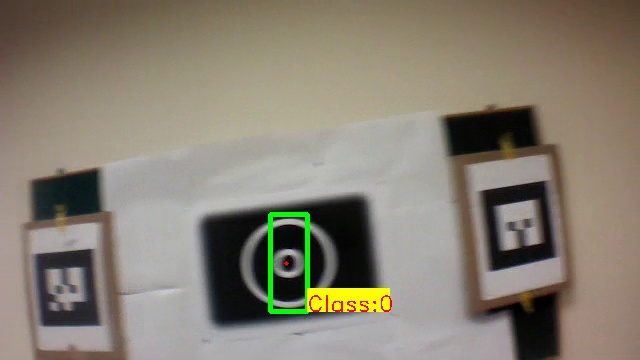
\includegraphics[width=\linewidth]{figures/fiducial/BLUT_input_00/output2.jpg}
\end{subfigure}
\begin{subfigure}[b]{.19\textwidth}
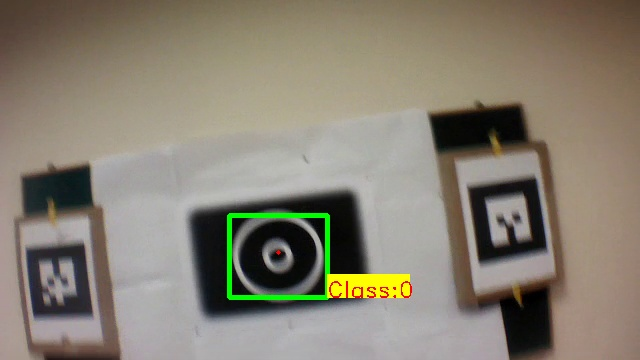
\includegraphics[width=\linewidth]{figures/fiducial/BLUT_input_00/output3.jpg}
\end{subfigure}
\begin{subfigure}[b]{.19\textwidth}
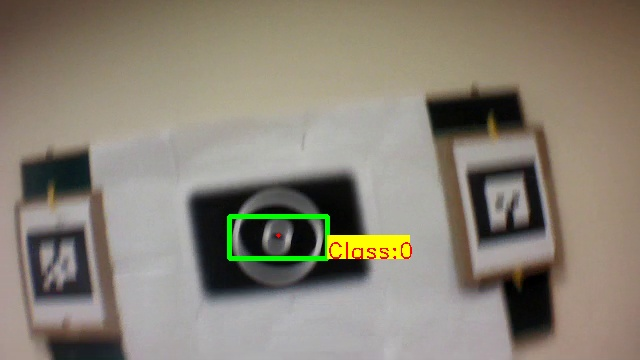
\includegraphics[width=\linewidth]{figures/fiducial/BLUT_input_00/output4.jpg}
\end{subfigure}
\begin{subfigure}[b]{.19\textwidth}
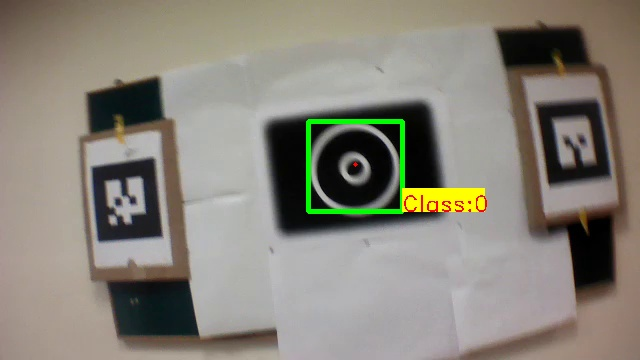
\includegraphics[width=\linewidth]{figures/fiducial/BLUT_input_00/output5.jpg}
\end{subfigure}
\begin{subfigure}[b]{.19\textwidth}
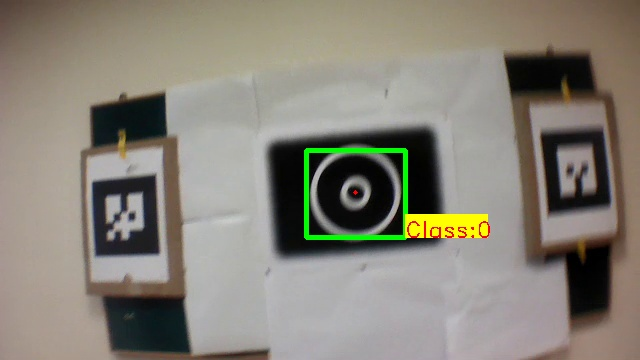
\includegraphics[width=\linewidth]{figures/fiducial/BLUT_input_00/output6.jpg}
\end{subfigure}
\caption[Output of BLUT on ARTag and our fiducial ``00'']{\textbf{Top:} Output of
BLUT~\cite{Wu:2011}.
\textbf{Bottom:} Output of our algorithm on the same image 
  sequence. BLUT is able to track the fiducial till the third frame,
  but from the fourth frame onwards, BLUT loses track. In the first
  three frames, the size of the  bounding box is low, but in the fourth
  and fifth frame it is large, indicating a sudden forward movement
  of the quadcopter.} 
\label{fig:BLUT_compare_00}
\end{figure*}

\begin{figure*}
\begin{subfigure}[b]{.19\textwidth}
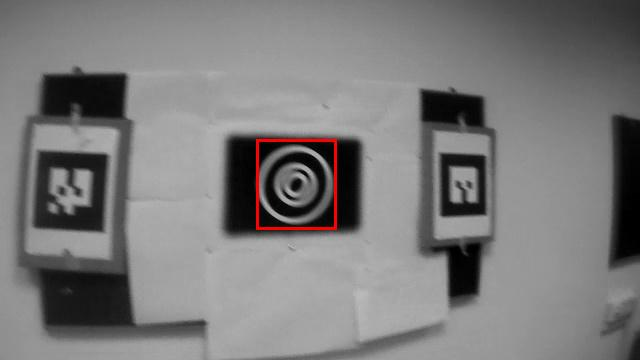
\includegraphics[width=\linewidth]{figures/fiducial/BLUT_output_01/11.jpg}
\end{subfigure}
\begin{subfigure}[b]{.19\textwidth}
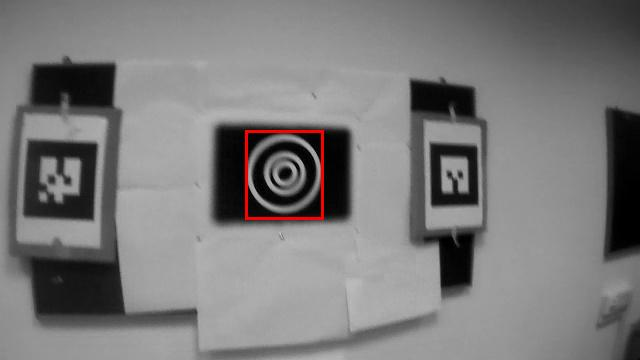
\includegraphics[width=\linewidth]{figures/fiducial/BLUT_output_01/12.jpg}
\end{subfigure}
\begin{subfigure}[b]{.19\textwidth}
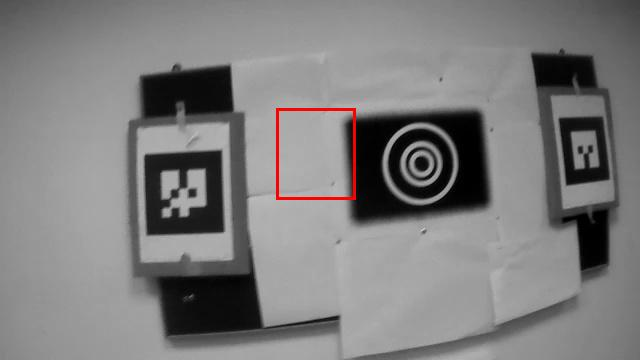
\includegraphics[width=\linewidth]{figures/fiducial/BLUT_output_01/13.jpg}
\end{subfigure}
\begin{subfigure}[b]{.19\textwidth}
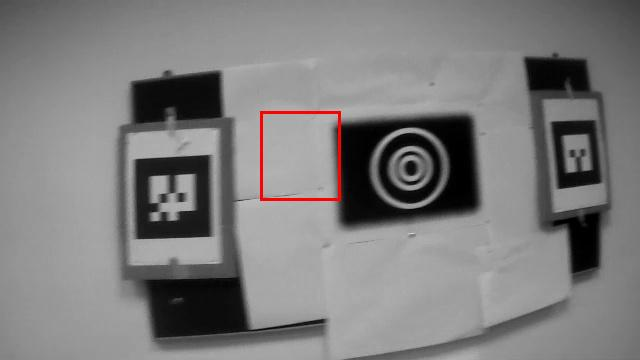
\includegraphics[width=\linewidth]{figures/fiducial/BLUT_output_01/14.jpg}
\end{subfigure}
\begin{subfigure}[b]{.19\textwidth}
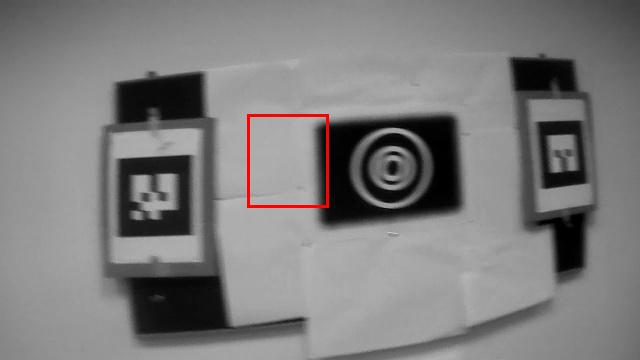
\includegraphics[width=\linewidth]{figures/fiducial/BLUT_output_01/15.jpg}
\end{subfigure}\\
\begin{subfigure}[b]{.19\textwidth}
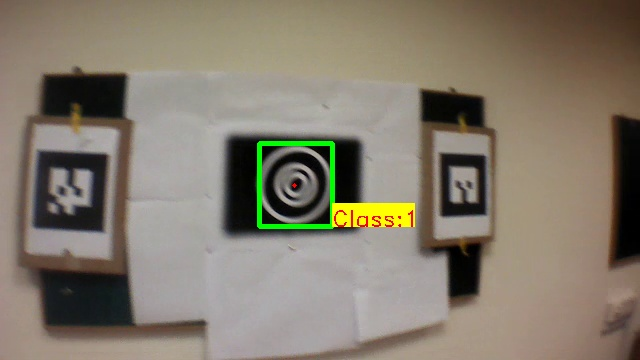
\includegraphics[width=\linewidth]{figures/fiducial/BLUT_input_01/output11.jpg}
\end{subfigure}
\begin{subfigure}[b]{.19\textwidth}
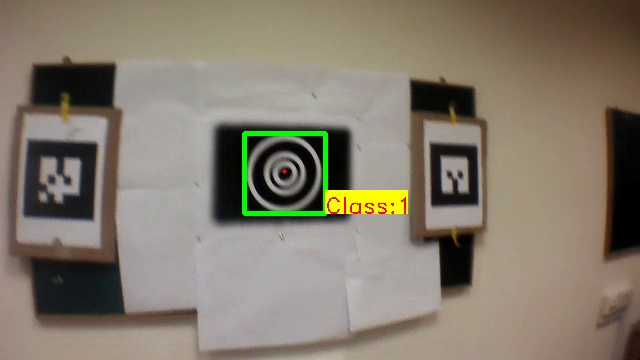
\includegraphics[width=\linewidth]{figures/fiducial/BLUT_input_01/output12.jpg}
\end{subfigure}
\begin{subfigure}[b]{.19\textwidth}
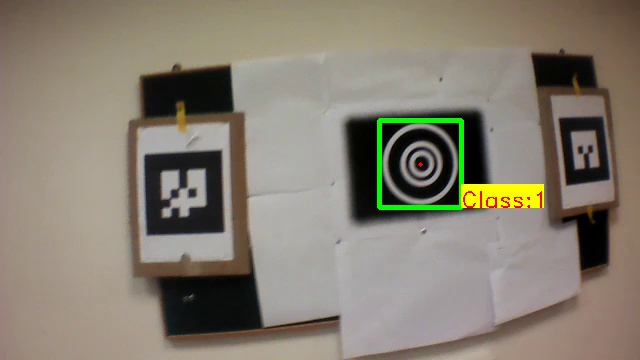
\includegraphics[width=\linewidth]{figures/fiducial/BLUT_input_01/output13.jpg}
\end{subfigure}
\begin{subfigure}[b]{.19\textwidth}
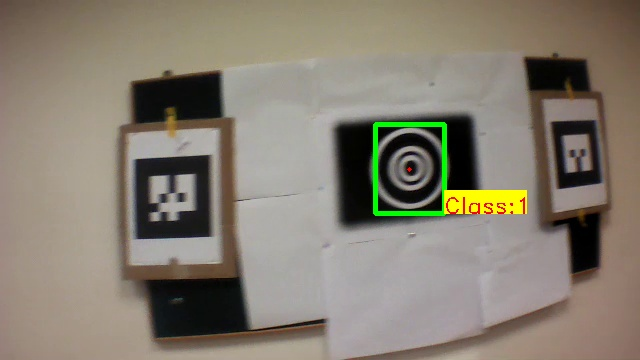
\includegraphics[width=\linewidth]{figures/fiducial/BLUT_input_01/output14.jpg}
\end{subfigure}
\begin{subfigure}[b]{.19\textwidth}
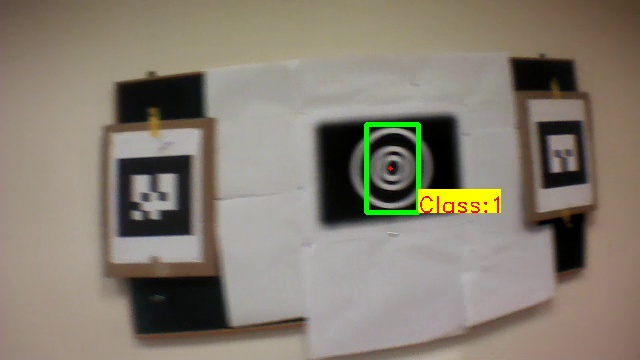
\includegraphics[width=\linewidth]{figures/fiducial/BLUT_input_01/output15.jpg}
\end{subfigure}
\caption[Output of BLUT on ARTag and our fiducial code ``01'']{{\bf Top:} Output of
BLUT~\cite{Wu:2011} on a sequence containing the ``01'' binary coded fiducial. {\bf Bottom:} Output of our
algorithm on the same image 
sequence. BLUT loses  track from the third frame onwards.}
\label{fig:BLUT_compare_01}
\end{figure*}

\begin{comment}
\begin{figure*}
\begin{subfigure}[b]{.19\textwidth}
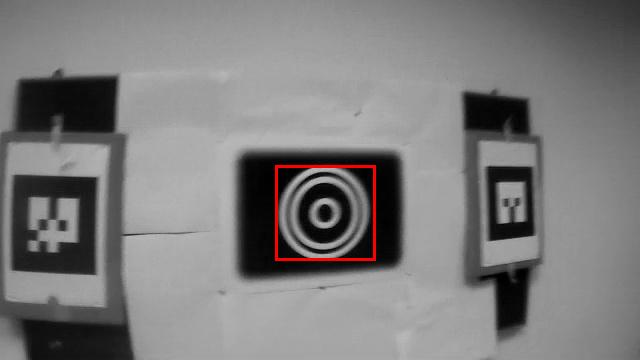
\includegraphics[width=\linewidth]{figures/fiducial/BLUT_output_10/1.jpg}
\end{subfigure}
\begin{subfigure}[b]{.19\textwidth}
\includegraphics[width=\linewidth]{figures/fiducial/BLUT_output_10/2.jpg}
\end{subfigure}
\begin{subfigure}[b]{.19\textwidth}
\includegraphics[width=\linewidth]{figures/fiducial/BLUT_output_10/3.jpg}
\end{subfigure}
\begin{subfigure}[b]{.19\textwidth}
\includegraphics[width=\linewidth]{figures/fiducial/BLUT_output_10/4.jpg}
\end{subfigure}
\begin{subfigure}[b]{.19\textwidth}
\includegraphics[width=\linewidth]{figures/fiducial/BLUT_output_10/5.jpg}
\end{subfigure}\\
\begin{subfigure}[b]{.19\textwidth}
\includegraphics[width=\linewidth]{figures/fiducial/BLUT_input_10/output1.jpg}
\end{subfigure}
\begin{subfigure}[b]{.19\textwidth}
\includegraphics[width=\linewidth]{figures/fiducial/BLUT_input_10/output2.jpg}
\end{subfigure}
\begin{subfigure}[b]{.19\textwidth}
\includegraphics[width=\linewidth]{figures/fiducial/BLUT_input_10/output3.jpg}
\end{subfigure}
\begin{subfigure}[b]{.19\textwidth}
\includegraphics[width=\linewidth]{figures/fiducial/BLUT_input_10/output4.jpg}
\end{subfigure}
\begin{subfigure}[b]{.19\textwidth}
\includegraphics[width=\linewidth]{figures/fiducial/BLUT_input_10/output5.jpg}
\end{subfigure}
\caption{Top: Output of BLUT~\cite{Wu:2011} on sample image sequence containing
``10'' binary coded fiducial. Bottom: Output of our algorithm on the same image
sequence. From the second frame, BLUT loses track.}
\label{fig:BLUT_compare_10}
\end{figure*}

\begin{figure*}
\begin{subfigure}[b]{.19\textwidth}
\includegraphics[width=\linewidth]{figures/fiducial/BLUT_output_11/2.jpg}
\end{subfigure}
\begin{subfigure}[b]{.19\textwidth}
\includegraphics[width=\linewidth]{figures/fiducial/BLUT_output_11/3.jpg}
\end{subfigure}
\begin{subfigure}[b]{.19\textwidth}
\includegraphics[width=\linewidth]{figures/fiducial/BLUT_output_11/4.jpg}
\end{subfigure}
\begin{subfigure}[b]{.19\textwidth}
\includegraphics[width=\linewidth]{figures/fiducial/BLUT_output_11/5.jpg}
\end{subfigure}
\begin{subfigure}[b]{.19\textwidth}
\includegraphics[width=\linewidth]{figures/fiducial/BLUT_output_11/6.jpg}
\end{subfigure}\\
\begin{subfigure}[b]{.19\textwidth}
\includegraphics[width=\linewidth]{figures/fiducial/BLUT_input_11/output2.jpg}
\end{subfigure}
\begin{subfigure}[b]{.19\textwidth}
\includegraphics[width=\linewidth]{figures/fiducial/BLUT_input_11/output3.jpg}
\end{subfigure}
\begin{subfigure}[b]{.19\textwidth}
\includegraphics[width=\linewidth]{figures/fiducial/BLUT_input_11/output4.jpg}
\end{subfigure}
\begin{subfigure}[b]{.19\textwidth}
\includegraphics[width=\linewidth]{figures/fiducial/BLUT_input_11/output5.jpg}
\end{subfigure}
\begin{subfigure}[b]{.19\textwidth}
\includegraphics[width=\linewidth]{figures/fiducial/BLUT_input_11/output6.jpg}
\end{subfigure}
\caption{Top: Output of BLUT~\cite{Wu:2011} on sample image sequence containing
``11'' binary coded fiducial. Bottom: Output of our algorithm on the same image
sequence. BLUT lost the track from third frame. There is sudden reversal of
direction from the quadcopter in the third frame. In first two frames, the quadcopter was
going up, but suddenly moved down.}
\label{fig:BLUT_compare_11}
\end{figure*}
\end{comment}

\section{Discussion and Limitations}\label{sec:discussion}

We have demonstrated the effectiveness of our blur invariant fiducial
both on synthetic data, and on real video clips captured from a quadcopter.
Our approach obtains a recognition rate of 86\%--95\% 
in real scenes compared to existing methods that average around
64\%.  We discuss some limitations of our approach in this section.
%\noindent\textbf{Processing Time}~~

Our  current processing time (0.3 seconds per frame) does not provide
real-time performance.  As such, we envision the method will be used in an
offline manner for performing analysis of flight paths. Code profiling revealed
that the Gabor filtering along the eight directions takes most of the time
(0.03 -- 0.04 seconds per orientation).  Either an improved Gabor filter scheme
is required or an alternative strategy for detection is required.
%\noindent\textbf{False Negatives}~~

We found that sometimes our detection algorithm fails to recognize the
``00'' fiducial, when there is severe blur.  This is because when there
is too much blur, the innermost ring's response in the Gabor output is
too low and not detected properly.  This problem can be resolved by
increasing the radius of innermost ring to reduce the effect of blur
on the innermost ring.
%\noindent\textbf{Pose Estimation}~~

We note that other markers are able to give full pose estimation after
detection.  However, we are only able to reliably detect the center
point and therefore cannot estimate pose.  Of course, if four markers
were used in a known order, pose could be estimated. The current
resolution of onboard camera is a significant  hurdle to clear before we
can effectively use multiple markers in each scene.
%\noindent\textbf{Number of Fiducials}~~

In terms of numbers of fiducials, we are able to generate less markers
than ARTag. Many applications in robotics (e.g., quadcopter navigation)
may not require simultaneous use of a large number of fiducials.  Most
of the time, it is sufficient to have 4-6 different
fiducials. Nevertheless, we may be able to generate a larger number of
fiducials by using color backgrounds. This is an area of interest for
further research.

\section{Conclusion}

Quadcopters are subject to quick and unstable motions that can cause
significant motion blur in the captured images. This severely affects
the detection rate of existing fiducials. We proposed the
design of a fiducial that is resistant to motion blur. Our design of
contrasting concentric rings is based on the observation that the
direction perpendicular to the motion blur direction will be
unaffected by the blur and therefore still be recognizable. We have
shown through experimental validation that our fiducial will work
under large amounts of motion blur and can significantly outperform
existing fiducials under this scenario.

\label{ch:fiducial}